% Compile with pdflatex main.tex
% Run with evince main.pdf
\documentclass[a4paper,12pt]{article}

\usepackage{lmodern}
\usepackage[T1]{fontenc}
% Adatta Latex alle convenzioni tipogafiche italiane
\usepackage[italian]{babel} 
% Consente l'uso dei caratteri accentati italiani
\usepackage[utf8]{inputenc}
% Simboli matematici (if we need) 
\usepackage{amsmath}
\usepackage{amsthm}
% Scrittura di codici
\usepackage{listings}
% Altri package di utilità generica
\usepackage{titling}
\usepackage{color}
\usepackage{graphicx}
\usepackage{caption}
\usepackage{wallpaper}
\usepackage{hyperref} 

% Impostazioni dei codici
\lstset{
breaklines=true,
basicstyle=\footnotesize,
frameshape={RYR}{Y}{Y}{RYR}} 

% Definizione del comando subtitle
\newcommand{\subtitle}[1]{
  \posttitle{
    \par\end{center}
    \begin{center}\large#1\end{center}
    \vskip0.5em}
}

% Definizione dell'intestazione
\title{Implementazione di una chat in linguaggio Java con crittografia asimmetrica}
\subtitle{Progetto del corso di Reti di Calcolatori}
\author{Valentino Marano, Amerigo Mancino}
\date{Giugno 2015}

% Documento principale
\begin{document}

% Creo la prima pagina
\maketitle

% Elimino il numero di pagina dalla copertina
\thispagestyle{empty}

% Logo dell'università
\begin{figure}[!bth]

\includegraphics[width=3.0cm]{logo.jpg} 
\centering
\end{figure}

% Indice
\newpage
\tableofcontents
\newpage

% Importo le varie parti del documento
\section{Presentazione degli obiettivi}
Il nostro progetto per il corso di Reti di Calcolatori si è concentrato sullo sviluppo
di una applicazione di messaggistica per reti locali (LAN).
Si è progettato il programma in modo tale da
sfruttare il protocollo UDP per lo scambio dei messaggi, i quali si ipotizzano essere criptati tramite
crittografia asimmetrica con chiave pubblica/privata. Per di più, l'applicazione
è stata pensata per essere in grado di inviare anche allegati (che definiamo, a questo proposito,
come file generici quali immagini, audio, etc), anch'essi criptati.
Il programma, teoricamente, deve essere in grado di identificare tutti gli utenti connessi
alla LAN, così da rendere possibile scegliere con quale utente si desidera chattare,
similmente a quanto avviene con applicazioni note quali Skype o Telegram Desktop.
Inoltre deve godere di un'interfaccia grafica intuitiva per semplificare
le operazioni.

\section{Progetti a confronto}
L'idea della chat non è di certo innovativa. Ne esistono di molti tipi da diversi anni e
ognuna di loro ha manifestato il proprio momento di gloria, per poi abbandonare i riflettori
e dirigere gli utenti verso applicazioni più nuove e immediate.

Nell'ambito dei progetti realizzati in passato per il corso di Reti di Calcolatori,
in particolare, nel 2006 uno studente ha proposto un servizio di messaggistica su
connessione cifrata con SSL ad architettura p2p, non realizzando tuttavia tutte le premesse
e abbandonando quindi l'implementazione della cifratura con SSL e, di conseguenza,
la gestione dei certificati. Questo lavoro era stato svolto sfruttando la libreria Axis
di Apache Foundation.

Nel 2014 altri due studenti hanno realizzato una chat prevedendo un'unità centrale che
potesse immagazzinare i dati strettamente necessari sugli utenti, senza quindi affidare dati
ridondanti a tutti i client. Il loro obiettivo era quello di creare un servizio che fosse
a metà fra le chat peer to peer e le chat centralizzate.

\newpage
\section{Sviluppo degli Obiettivi}
Quasi tutte le parti poste nella Presentazione degli Obiettivi sono state correttamente
sviluppate e implementate. La chat realizzata possiede una GUI per l'interazione
con l'utente avente il seguente aspetto:
\begin{figure}[h]
\centering
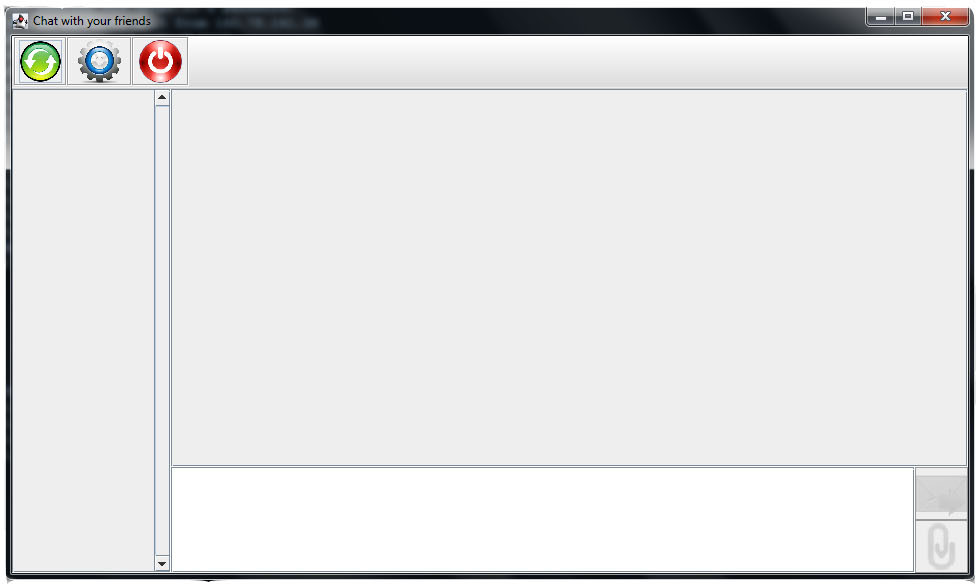
\includegraphics[scale=0.4]{gui1.jpg}
\label{fig:gui}
\end{figure}

Il riquadro in basso permette la scrittura di testo.
I due tasti laterali ad esso affiancati
consentono invece di inviare messaggi (criptati) o allegati (non criptati).
In alto sono presenti tre bottoni:
di essi, quello più a sinistra consente di scandire la rete per la ricerca di eventuali 
utenti che, in questo momento, stanno utilizzando la chat, tali utenti vengono salvati
in una lista di utenti conosciuti.
Tale scansione viene in ogni caso eseguita in automatico all'avvio del programma
e ripetuta periodicamente durante la sua esecuzione per aggiornare tale lista.
Quando un utente viene trovato, nel riquadro a sinistra 
dell'applicazione viene inserito un pulsante con il suo nickname.
Cliccandoci sopra, diventa possibile chattare con lui e inviargli messaggi.
Il bottone al centro, invece, apre un'altra piccola finestra.

\begin{figure}[h]
\centering

\includegraphics[scale=0.3]{settings.png}
\end{figure}

Questa finestra gestisce le impostazioni e da qui l'utente può regolare:
\begin{itemize}
	\item ogni quanti secondi far eseguire la scansione della rete
	\item ogni quante scansioni svuotare completamente l'insieme degli host conosciuti 
	in modo da non conservare inutilmente host non più presenti nella LAN o che abbiano
	chiuso l'applicazione.
	\item cambiare il suono di notifica che verrà riprodotto all'arrivo di un messaggio	
\end{itemize}
Il pulsante mentre quello più a destra consente di chiudere l'applicazione, prima della
chiusura verrà mostrato un messaggio di conferma per chiedere all'utente se vuole chiudere
l'applicazione. Prima di essere chiusa l'applicazione manda a tutti gli host conosciuti
un messaggio speciale \emph{\#\#DOWN\#\#} in modo che gli altri host sulla LAN sappiano che si
sta disconnettendo e lo tolgano subito dalla lista degli host conosciuti.
All'avvio del programma si cerca il file di configurazione e si cerca di
leggere il nome utente e le impostazioni. In caso non venga trovato il file o il nome utente
non sia presente (è il primo accesso fatto dall'utente) compare una schermata di login:
\begin{figure}[h]
\centering
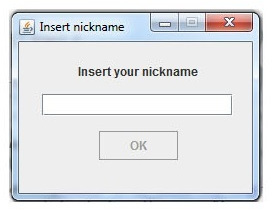
\includegraphics[scale=0.5]{login1.jpg}
\label{fig:login}
\end{figure}

In questa scheda l'utente crea il proprio account, scegliendo un nickname da usare in chat.
Una volta digitato il nickname, il tasto di conferma diventa cliccabile e premendolo si effettua
il login ed è possibile iniziare ad usare l'applicazione.
Viene poi controllata la presenza della coppia di chiavi e nel caso non siano presenti vengono create.

In questa relazione, analizzeremo a grandi linee la codifica proposta e l'implementazione
delle varie classi, con particolare enfasi sul ruolo giocato da ognuna di esse.
Mostreremo, poi, i risultati ottenuti e, infine,
il funzionamento dell'intero programma qui presentato,
esponendo anche i test fatti in corso d'opera
in locale e sulla Virtual Private Network di ateneo.
Il lavoro svolto sarà, quindi, accompagnato dalle dovute conclusioni e
da un commento sui possibili sviluppi futuri.
\section{Il package app}
Il package \texttt{app} contiene tutte e sole le classi che si occupano del corretto
funzionamento dell'applicazione, a partire dalla definizione della schermata di login
fino ad arrivare alla gestione delle chiavi. Analizzeremo nei prossimi sotto-paragrafi
le diverse classi nel dettaglio, presentandone i diversi metodi implementati.

\subsection{La classe Main}
La classe \texttt{Main} è la classe principale dell'applicazione.
Si occupa di lanciare il programma eseguendo \texttt{run},
ammesso che l'utente abbia effettuato il login in questa
o in una precedente sessione.
In caso contrario, viene fatto scegliere all'utente un nickname da usare nella chat
mediante il pannello grafico mostrato in precedenza e,solo dopo questa operazione,
l'applicazione può essere correttamente utilizzata.

\subsection{La classe App}
La classe \texttt{App} è la classe che si occupa della creazione e della gestione della
finestra grafica della chat. I metodi presenti sono i seguenti:
\section{Il package net}
Nel package \texttt{net} sono organizzate tutte le classi che si occupano di effettuare e gestire lo
scambio dei messaggi e di ricercare altri utenti nella rete.

\subsection{Ricerca di utenti}
La classe che si occupa della scansione è la classe \texttt{scan}. Per effettuare la
ricerca viene utilizzato \texttt{Nmap} (\url{http://nmap.org/}),  un software libero distribuito con licenza GNU GPL
creato originariamente per effettuare port scanning, cioè mirato all'individuazione di porte aperte
su un computer bersaglio o anche su range di indirizzi IP, in modo da determinare quali
servizi di rete siano disponibili. Un tipico esempio dell'uso di \texttt{Nmap} è il seguente:

\begin{lstlisting}
nmap www.google.it

Starting Nmap 6.40 ( http://nmap.org ) at 2015-06-05 09:47 CEST
Nmap scan report for www.google.it (74.125.206.94)
Host is up (0.026s latency).
Not shown: 998 filtered ports
PORT    STATE SERVICE
80/tcp  open  http
443/tcp open  https
\end{lstlisting}

Nello specifico, poi, per quanto concerne la nostra applicazione, \texttt{Nmap}
viene utilizzato principalmente per individuare chi utilizza il servizio di messaggistica.
Per eseguire \texttt{Nmap} viene adoperata la classe \texttt{Process} di Java.
Quando viene avviata una nuova scansione, tutte le coppie
$$ \langle \text{Nickname,indirizzo} \rangle $$
trovate vengono salvate e mostrate nella barra laterale sinistra della GUI, come già
anticipato sopra.

\subsection{Scambio di messaggi}
Lo scambio di messaggi non sfrutta, come si è intuito dai paragrafi precedenti un'architettura
client-server, ma il peer-to-peer. Fondamentalmente, tutti i nodi sono equivalenti e possiedono
un server sempre in ascolto per la ricezione dei messaggi ed un client predisposto, invece, all'invio
dei messaggi stessi. Abbiamo creato dunque una classe \texttt{Message} che implementa l'ADT
\textit{messaggio}, contenente fondamentalmente un campo di tipo stringa per il testo, un campo
per la data e un capo \texttt{tipo} posto a $0$ se il messaggio è ricevuto e posto a $1$ se inviato.

Lo scambio vero e proprio è implementato invece nelle classi \texttt{Chat\char`_manager} e \texttt{Server},
cuore dell'intero programma. Nella prima vengono settati i suoni, avviato il server, avviata la scansione
con \texttt{Nmap} della rete locale, aggiunti eventuali altri utenti che usano la chat, etc. Inoltre
è presente l'indispensabile metodo \texttt{send} che invia messaggi con Datagram Socket. Ad ogni
invio segue un acknowlegement di conferma di avvenuta ricezione.
Il metodo \texttt{attach} invece consente la gestione corretta degli allegati: un file viene, di
fatto, convertito in un flusso di byte, inglobato in Datagram Socket e inviato senza essere stato cifrato.

La classe \texttt{Server}, d'altro canto, ha come scopo principale quello di avviare il server
inizializzando poi un campo myIP e permettendo dunque ad altri utenti di poterlo identificare.
Dopodiché si addormenta, mettendosi in attesa di messaggi.
\section{Conclusioni e sviluppi futuri}
Il lavoro svolto ha permesso un completo sviluppo di un'applicazione di
messaggistica pienamente funzionante e operativa su reti locali. I test
fatti in locale e su VPN hanno dato risultati soddisfacenti permettendo un
pieno scambio di messaggi e file (si è testato, ad esempio, l'invio di
una semplice immagine). L'uso dell'interfaccia grafica realizzata con
SWING - siamo certi - permette una visualizzazione rapida dei messaggi
e semplifica molto l'uso dell'applicazione anche ad
utenti meno avvezzi all'uso di un terminale.

Nonostante l'applicazione abbia raggiunto una certa solidità,
numerosi sono i possibili interventi da attuare per migliorarla.
Sarebbe interessante criptare anche gli allegati oltre che i
messaggi al fine di garantire una maggiore riservatezza.
Inoltre i file contenenti le chat sono memorizzati sul PC
dell'utente in chiaro, il che li rende vulnerabili.
Di fatto, si potrebbero cifrare e decifrare ogni volta che viene chiamato
il metodo \texttt{openChat} (ossia ogni volta che viene premuto
un pulsante nella barra a sinistra dell'applicazione), introducendo
tuttavia in questo modo un overhead che, durante lo sviluppo, abbiamo
deciso di non aggiungere per non appesantire ulteriormente il programma.
Un altro problema presente che potrebbe essere risolto in futuro è il seguente:
la cronologia dei messaggi viene salvata, come detto precedentemente, in un
file
$$ \texttt{nickname.txt} $$
Questa decisione sta in piedi fintanto che non esistono due utenti con lo stesso nickname,
nel qual caso una sovrapposizione è inevitabile, portando alla perdita definitiva
di uno dei due storici. Una soluzione ipotizzata comporta l'inserimento di
un server centrale predisposto alla gestione dei nickname.
Altri miglioramenti attuabili riguardano poi prettamente l'interfaccia
grafica del programma, inserendo la possibilità di cambiare colori,
trasformando i messaggi in nuvolette, e così via.
\end{document}